\section{Derivatives computation}

Computation of derivative quantities such as gradient and Laplacian is of fundamental importance in
data analysis, so in this section, we studies streams that aim to minimize errors of derivative
fields. For the experiments in this section, instead of the CDF 5/3 linear B-spline wavelet, we use
the 4-4 B-spline wavelet [CITE] that has four vanishing moments on each of the analysis and
synthesis sides, to ensure that the reconstructed function is smooth enough for taking derivatives.
We also use quantize the original data to $32$ instead of $16$ bits, to avoid losing too much
precision due to floating-point cancellation in computing derivatives.

\subsection{Gradient}

Since simulation data can rarely be captured by closed-form formulas, we use finite difference to
compute the gradient. We experiment with three popular finite difference schemes using stencil sizes
of two, three, and five points, to compute partial derivatives in each direction: $\frac{\partial
f}{\partial x}\approx f(x+1)-f(x) \approx \frac{1}{2}f(x+1)-\frac{1}{2}f(x-1) \approx
\frac{1}{12}f(x-2)-\frac{2}{3}f(x-1)+\frac{2}{3}f(x+1)-\frac{1}{12}f(x+2)$. \hb{missing denominator $\partial x = 1$.. perhaps rename the stencil?} The gradient at each
grid point $(x,y)$ is the vector $(\frac{\partial f}{\partial x},\frac{\partial f}{\partial y})$. We
use algorithm (\Cref{sec:data_dep_streams} to compute a stream that minimizes the difference between
the gradient field of $f_b$ (the reconstructed function using $b$ bits per sample) and that of the
original function ($f$), defined as $\norm{\nabla f_b-\nabla f}_2$. This is called the
\emph{gradient-optimized} stream. For each of the three \emph{gradient-optimized} streams for the
three aforementioned stencils, we measure its gradient error against the analytically computed,
ground-truth gradient field of a $512\times 512$ synthetic function, $f(x,y)=\sin x\sin y$ for
$x,y\in[-0.5,0.5]$. The results are in Figure \ref{fig:gradient-error-comparison-stencils}.

\begin{figure}
	\centering
	\subcaptionbox{full}
	{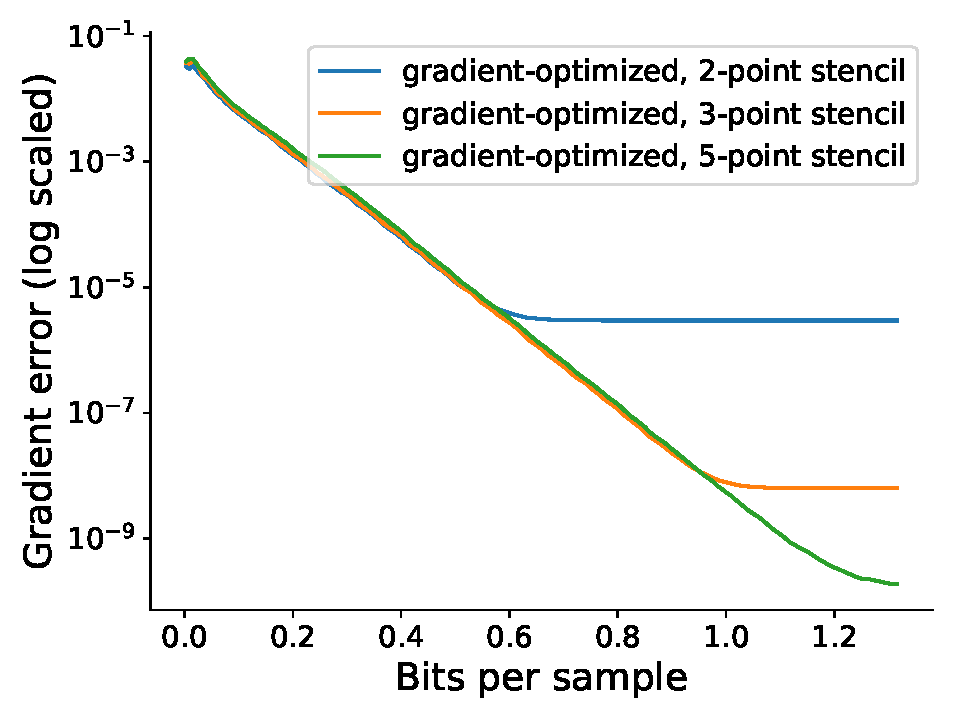
\includegraphics[width=0.48\linewidth]{img/gradient-laplacian/sine-gradient-stencils-full.pdf}}
	\subcaptionbox{zoomed in}
	{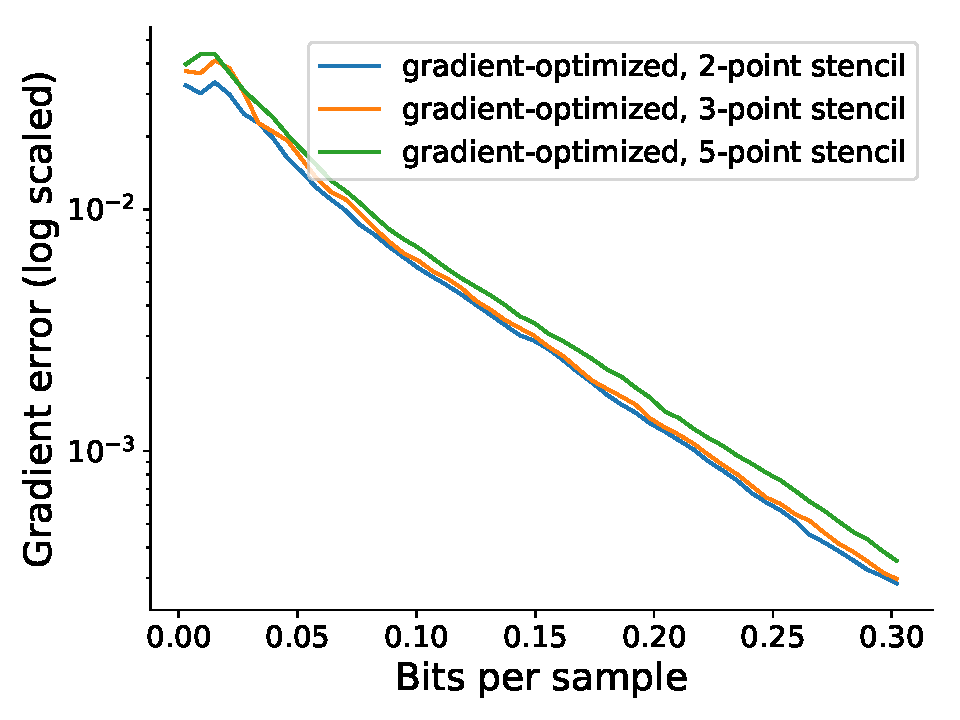
\includegraphics[width=0.48\linewidth]{img/gradient-laplacian/sine-gradient-stencils-cutoff.pdf}}
	\caption{Gradient error by three \emph{gradient-optimized} optimized	streams, using different
	 stencils. Smaller is better. The right plot zooms in on beginning part of the left plot, so as to
	 distinguish the curves. Smaller stencils perform marginally better at low bit rates, but fail to
	 track the ground-truth gradient at high bit rates.}
  \label{fig:gradient-error-comparison-stencils}
\end{figure}

At low bit rates, the two-point stencil performs the best, by a small margin. Its gradient error,
however, plateaus out the earliest, at about $0.6$ bits per sample, with an approximated error of
$10^-5$ (Figure \ref{fig:gradient-error-comparison-stencils}a). The three-point stencil achieves
effectively the same error as the two-point scheme, while achieving almost three orders of magnitude
smaller error at the maximum bit rate. The five-point scheme improves the error by another order of
magnitude, but suffers slightly more at low bit rates, possibly due to its larger size being more
susceptible to cancellation errors when subtracting low-precision floating-point values.
\hb{concise message is missing}

When comparing the \emph{gradient-optimized}, \emph{rmse-optimized} streams as well as their
data-independent analogues, \emph{gradient signature} and \emph{by wavelet norm} (Figure
\ref{fig:gradient-error-comparison}), we see that in the {fig:gradient-error-comparison} compares the \emph{gradient-optimized} with the
\emph{rmse-optimized} streams for four data sets.

\begin{figure}
	\centering
	\subcaptionbox{boiler, 3-point stencil}
	{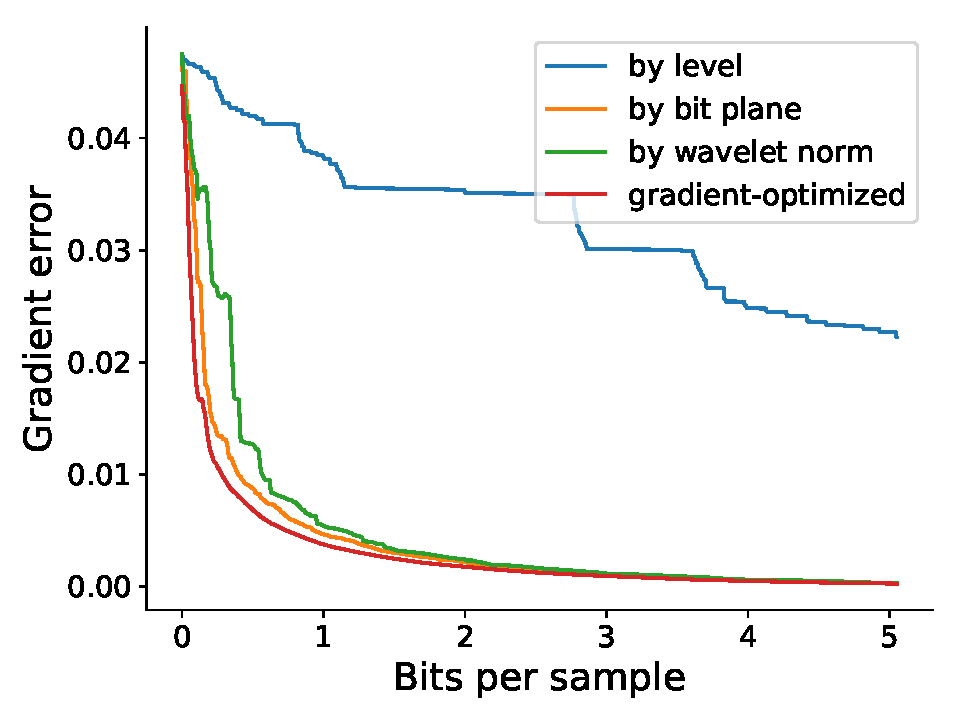
\includegraphics[width=0.48\linewidth]{img/gradient/3points/gradient-optimized-boiler.pdf}}
	\subcaptionbox{boiler, 5-point stencil}
	{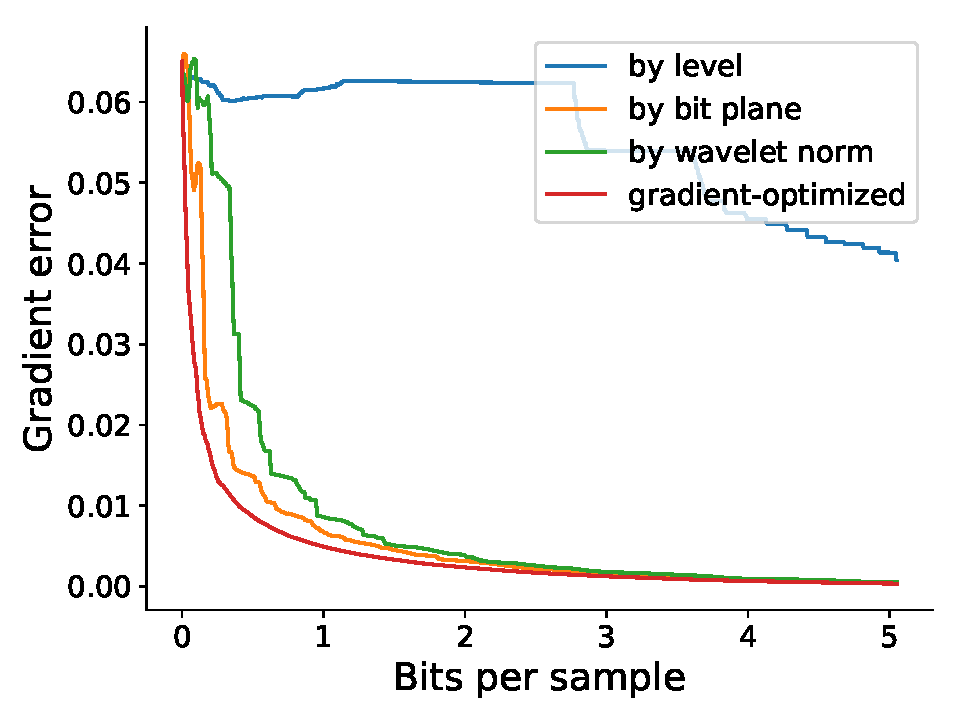
\includegraphics[width=0.48\linewidth]{img/gradient/5points/gradient-optimized-boiler.pdf}}
	\subcaptionbox{diffusivity, 3-point stencil}
	{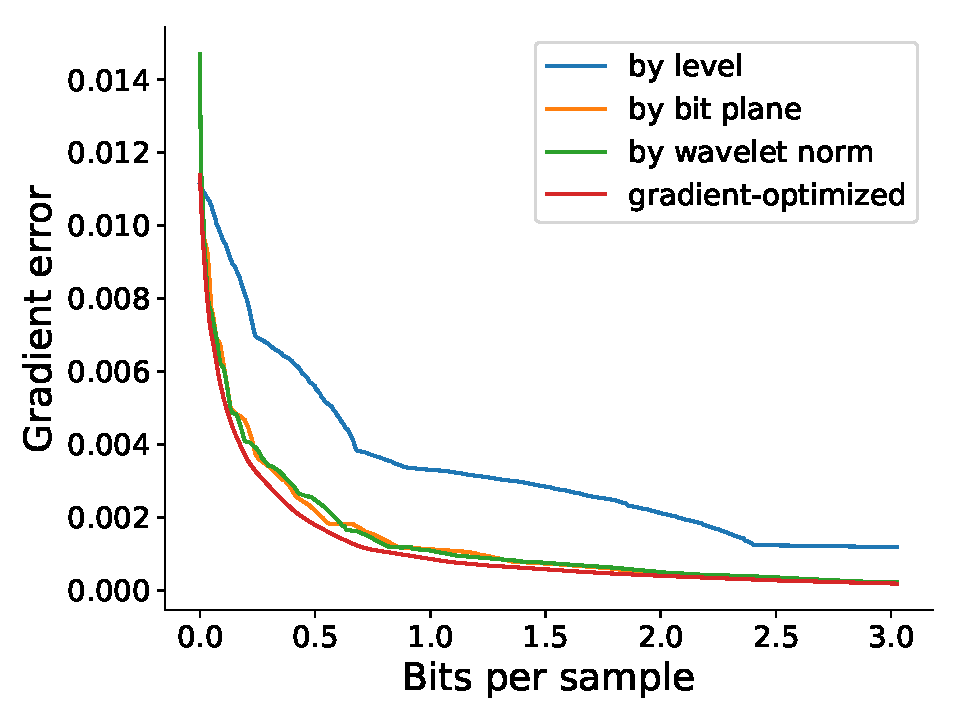
\includegraphics[width=0.48\linewidth]{img/gradient/3points/gradient-optimized-diffusivity.pdf}}
	\subcaptionbox{diffusivity, 5-point stencil}
	{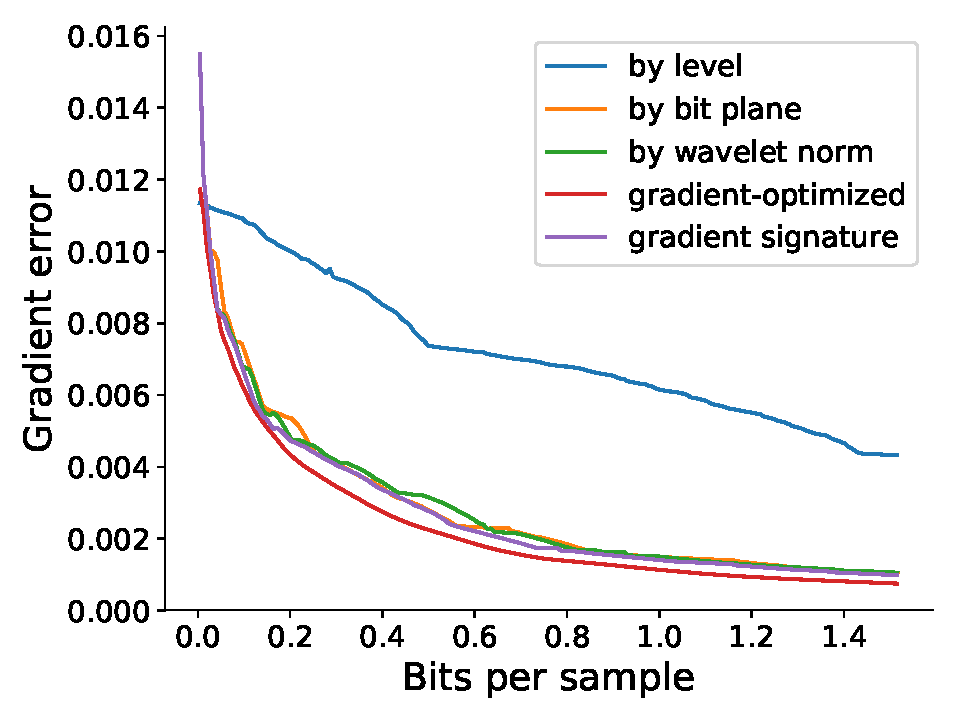
\includegraphics[width=0.48\linewidth]{img/gradient/5points/gradient-optimized-diffusivity.pdf}}
	\subcaptionbox{euler, 3-point stencil}
	{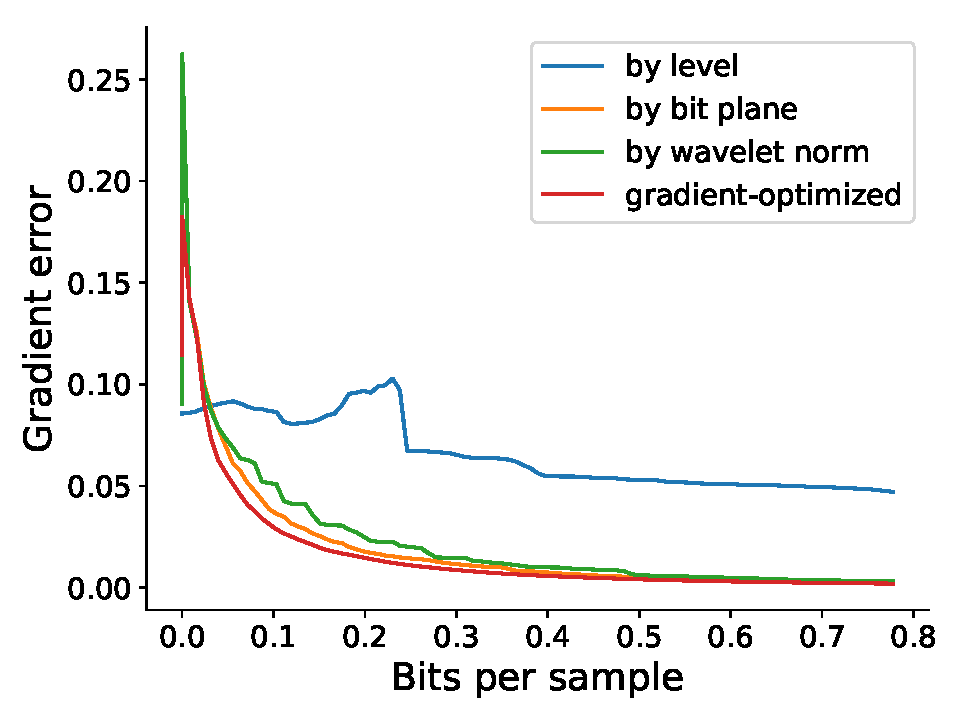
\includegraphics[width=0.48\linewidth]{img/gradient/3points/gradient-optimized-euler.pdf}}
	\subcaptionbox{euler, 5-point stencil}
	{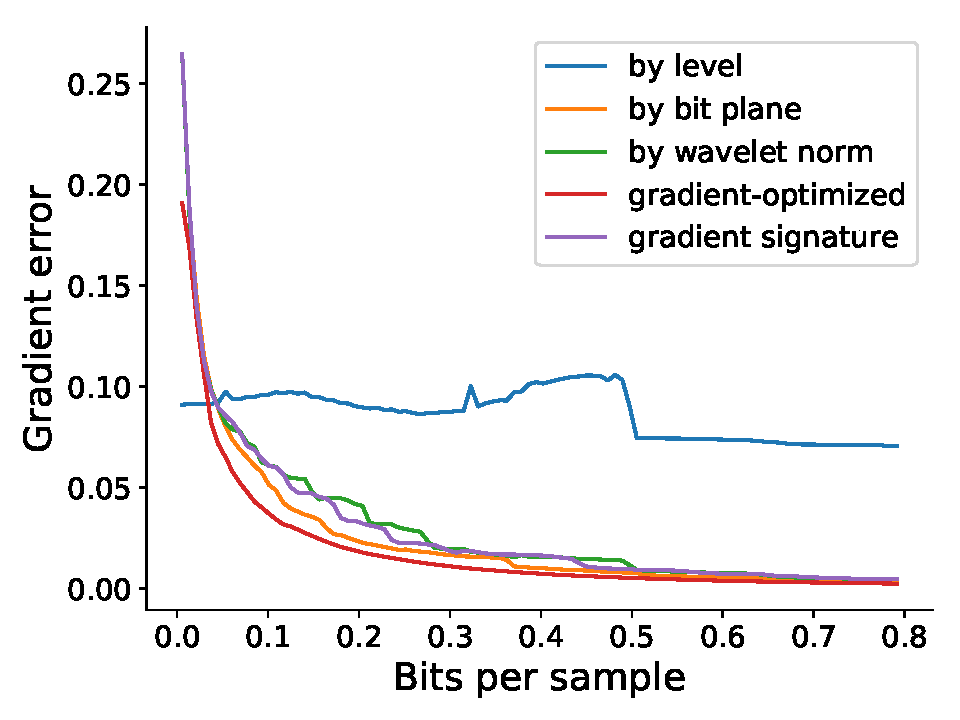
\includegraphics[width=0.48\linewidth]{img/gradient/5points/gradient-optimized-euler.pdf}}
	\subcaptionbox{marschner-lobb, 3-point stencil}
	{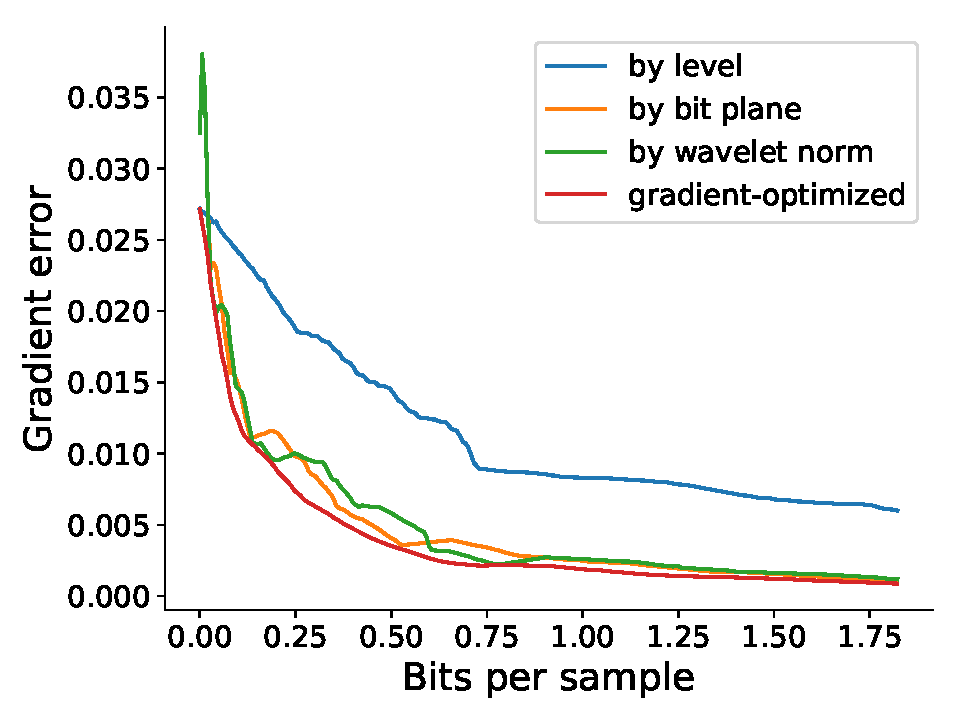
\includegraphics[width=0.48\linewidth]{img/gradient/3points/gradient-optimized-marschner-lobb.pdf}}
	\subcaptionbox{marschner-lobb, 5-point stencil}
	{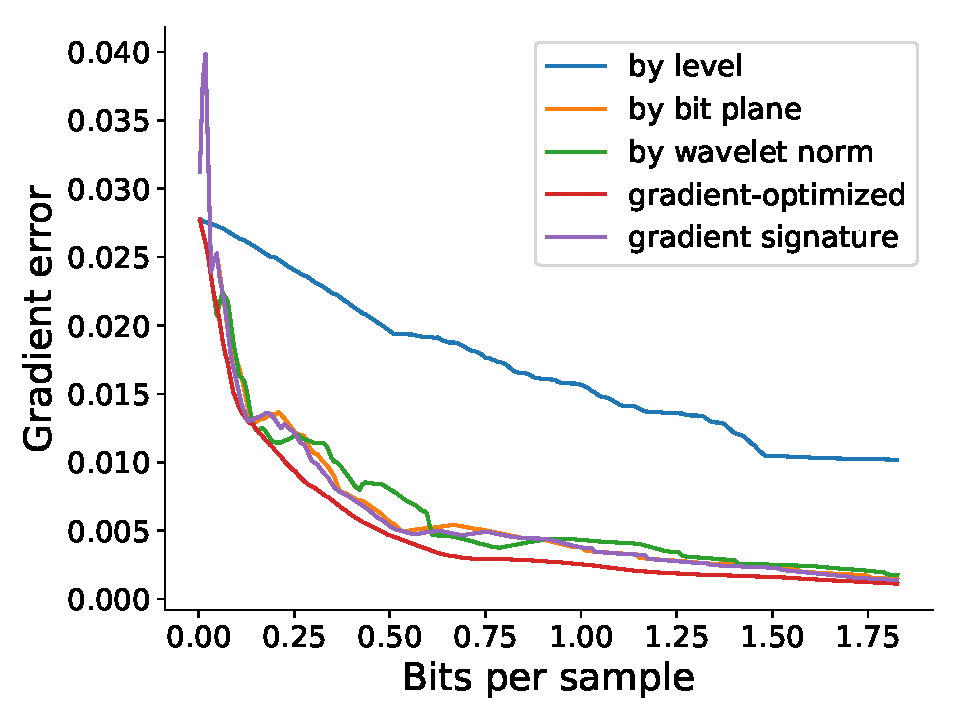
\includegraphics[width=0.48\linewidth]{img/gradient/5points/gradient-optimized-marschner-lobb.pdf}}
	\subcaptionbox{sinusoid, 3-point stencil}
	{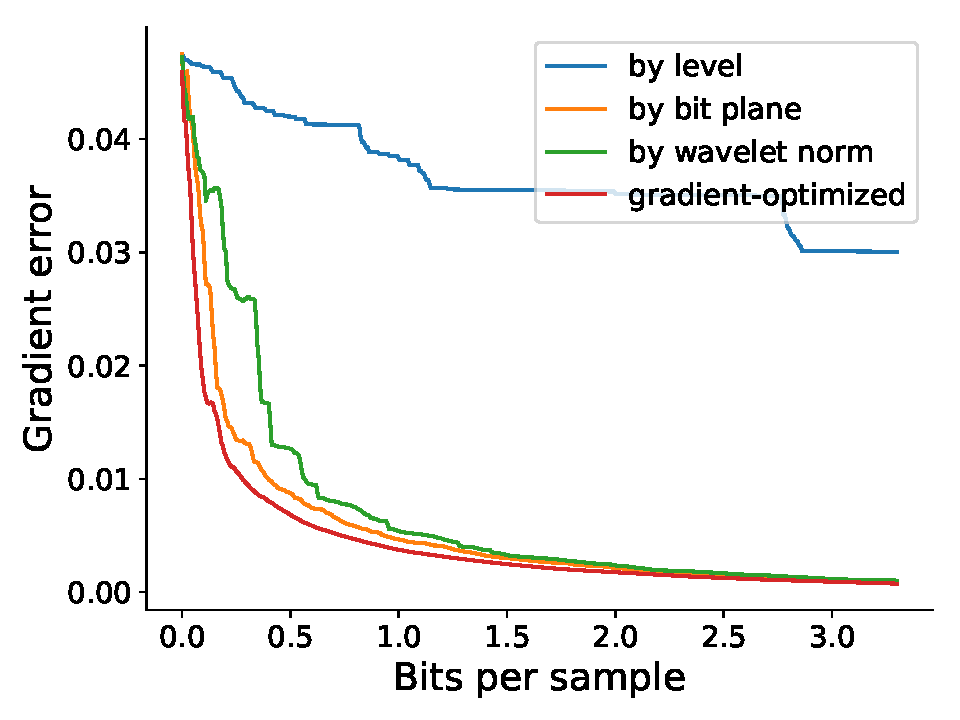
\includegraphics[width=0.48\linewidth]{img/gradient/3points/gradient-optimized-sinusoid.pdf}}
	\subcaptionbox{sinusoid, 5-point stencil}
	{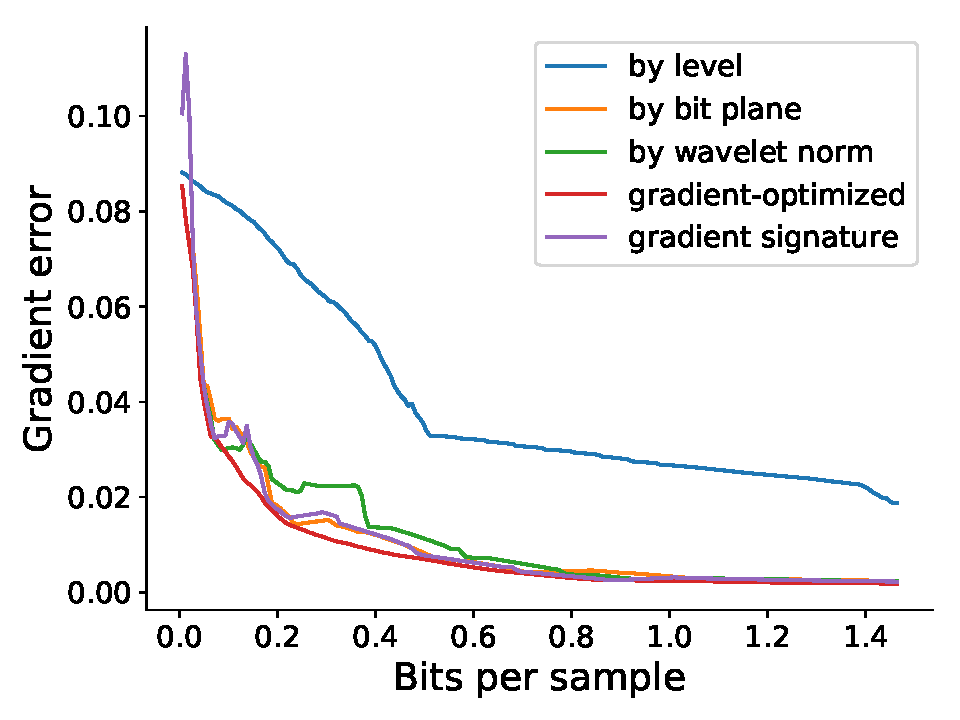
\includegraphics[width=0.48\linewidth]{img/gradient/5points/gradient-optimized-sinusoid.pdf}}
	\subcaptionbox{velocityz, 3-point stencil}
	{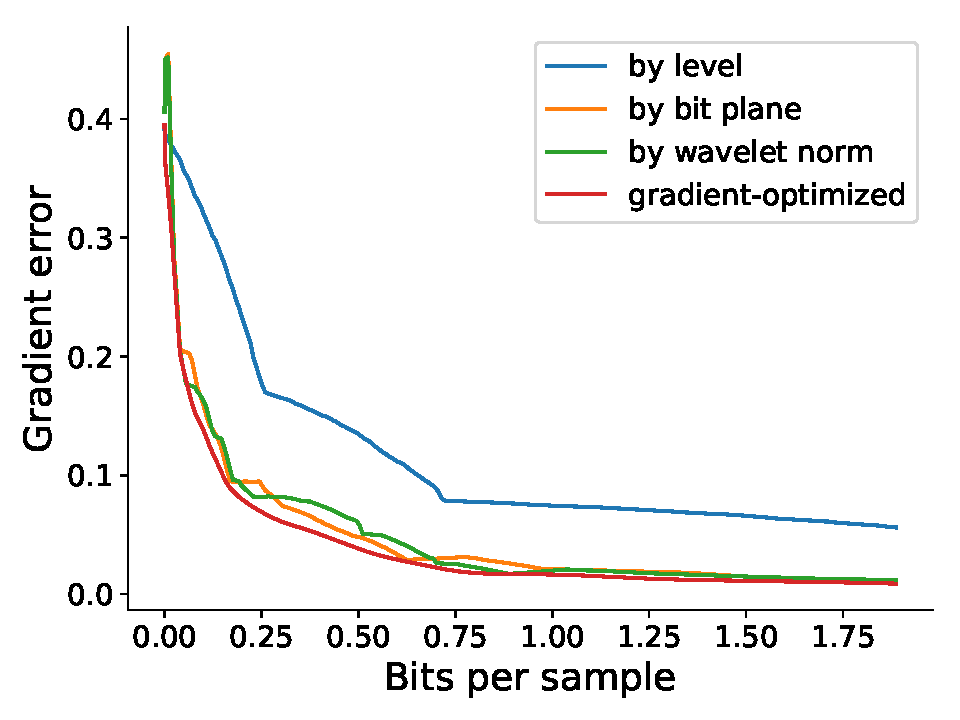
\includegraphics[width=0.48\linewidth]{img/gradient/3points/gradient-optimized-velocityz.pdf}}
	\subcaptionbox{velocityz, 5-point stencil}
	{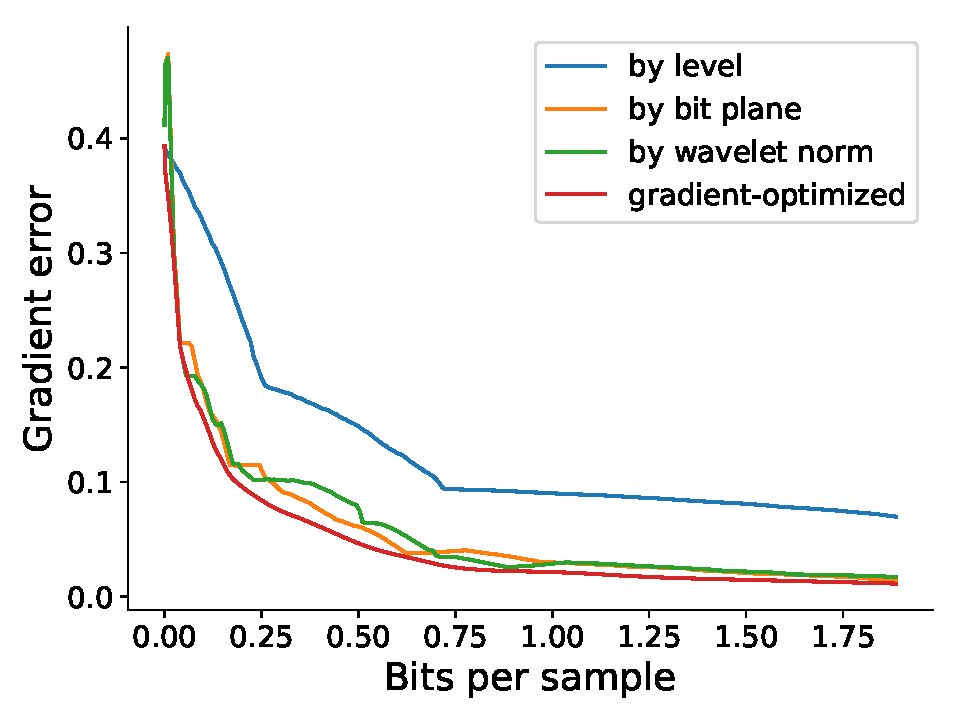
\includegraphics[width=0.48\linewidth]{img/gradient/5points/gradient-optimized-velocityz.pdf}}
	\caption{Gradient error comparison between \emph{gradient-optimized}, \emph{rmse-optimized},
	\emph{by wavelet norm}, and \emph{gradient signature} streams for four data sets, using the
	3-point stencil (left) and the 5-point stencil (right). Smaller is better. Chunks consisting of
	leading zero bits are removed from all streams. It all cases, the \emph{gradient-optimized} and
	\emph{rmse-optimized} streams perform the same, while \emph{gradient} signature is only slightly
	better than \emph{by wavelet norm}.}
	\label{fig:gradient-error-comparison}
\end{figure}

\begin{figure}
	\centering
	\subcaptionbox{euler, 3-point stencil}
	{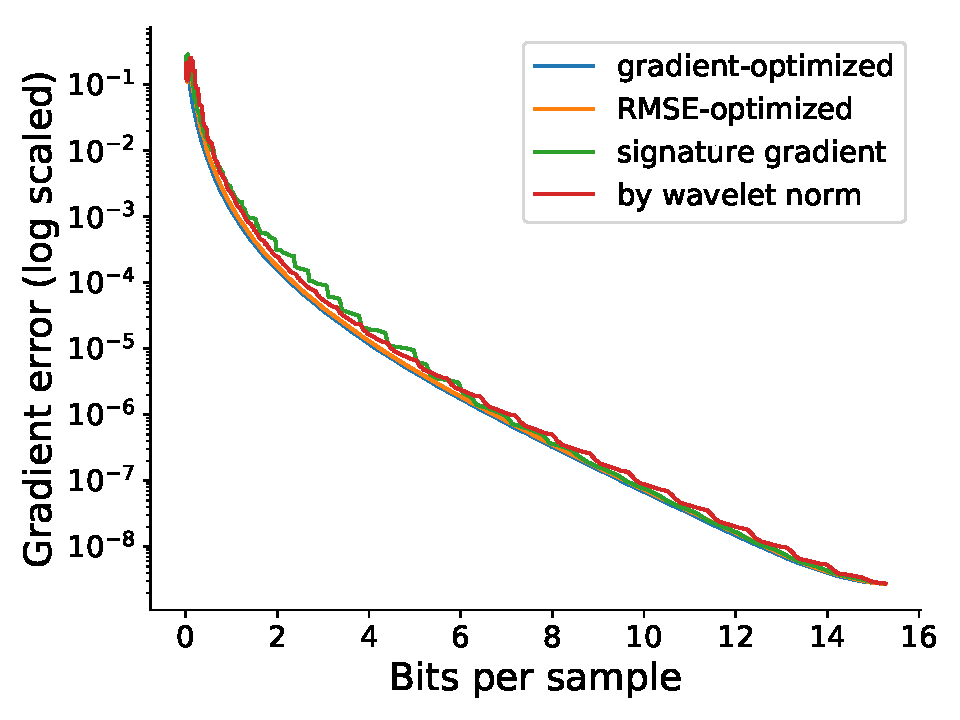
\includegraphics[width=0.48\linewidth]{img/gradient-laplacian/euler2d-gradient-stencil-3.pdf}}
	\subcaptionbox{euler, 5-point stencil}
	{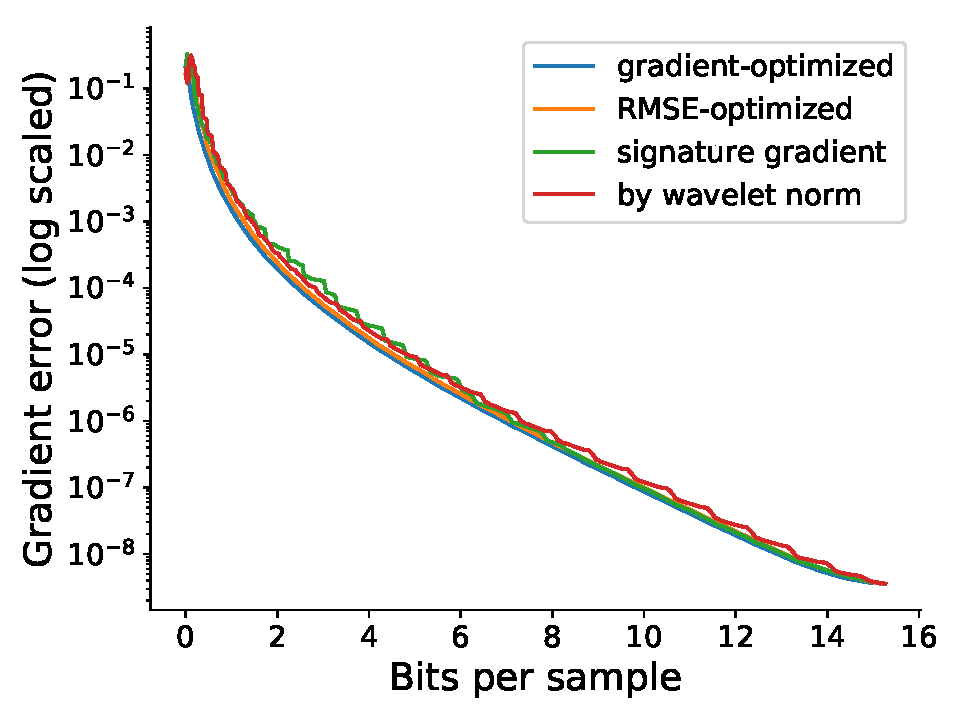
\includegraphics[width=0.48\linewidth]{img/gradient-laplacian/euler2d-gradient-stencil-5.pdf}}
	\subcaptionbox{magnetic, 3-point stencil}
	{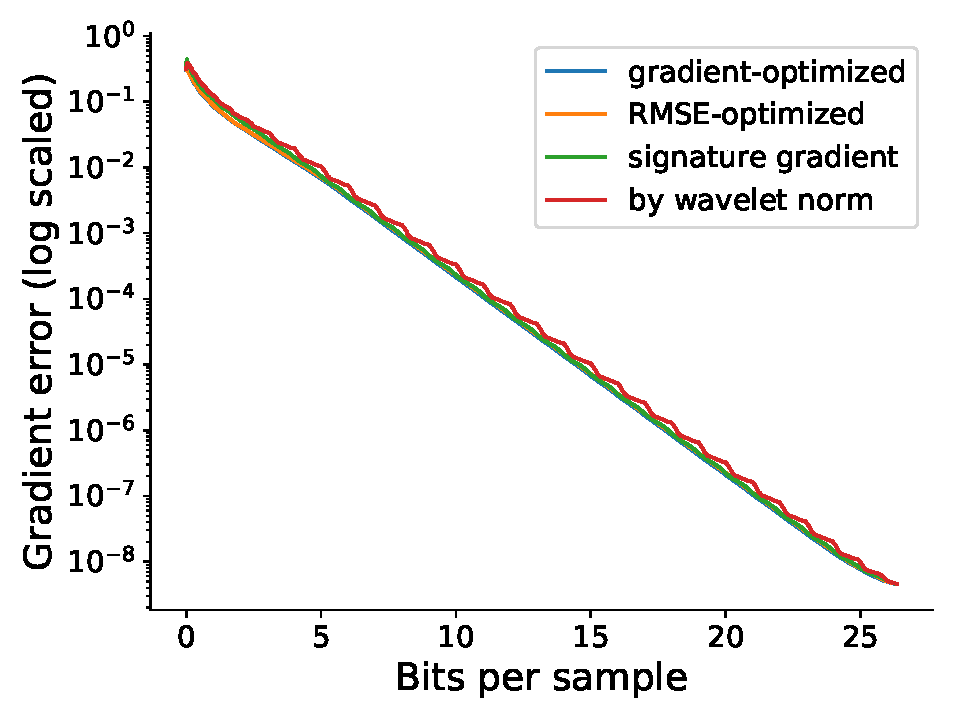
\includegraphics[width=0.48\linewidth]{img/gradient-laplacian/magnetic-gradient-stencil-3.pdf}}
	\subcaptionbox{magnetic, 5-point stencil}
	{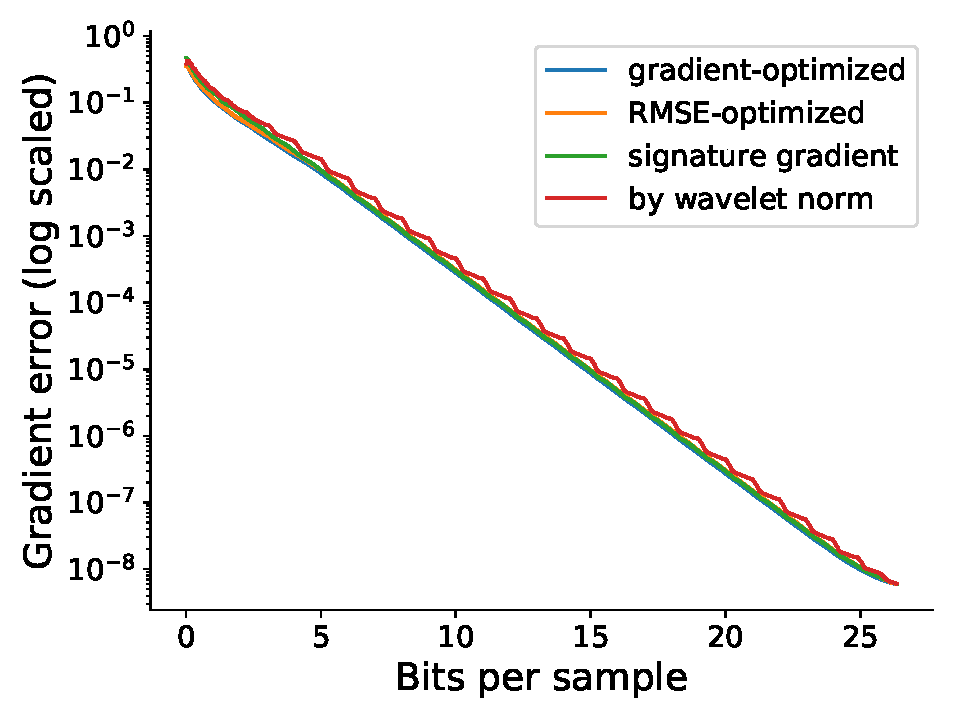
\includegraphics[width=0.48\linewidth]{img/gradient-laplacian/magnetic-gradient-stencil-5.pdf}}
	\subcaptionbox{diffusivity, 3-point stencil}
	{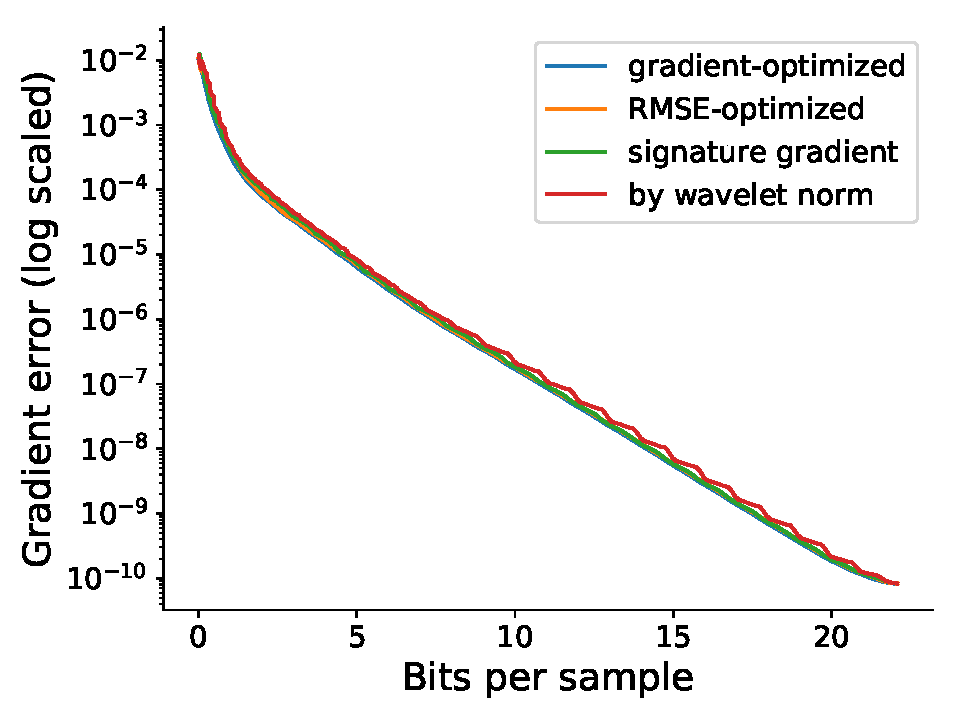
\includegraphics[width=0.48\linewidth]{img/gradient-laplacian/miranda-diffusivity-gradient-stencil-3.pdf}}
	\subcaptionbox{diffusivity, 5-point stencil}
	{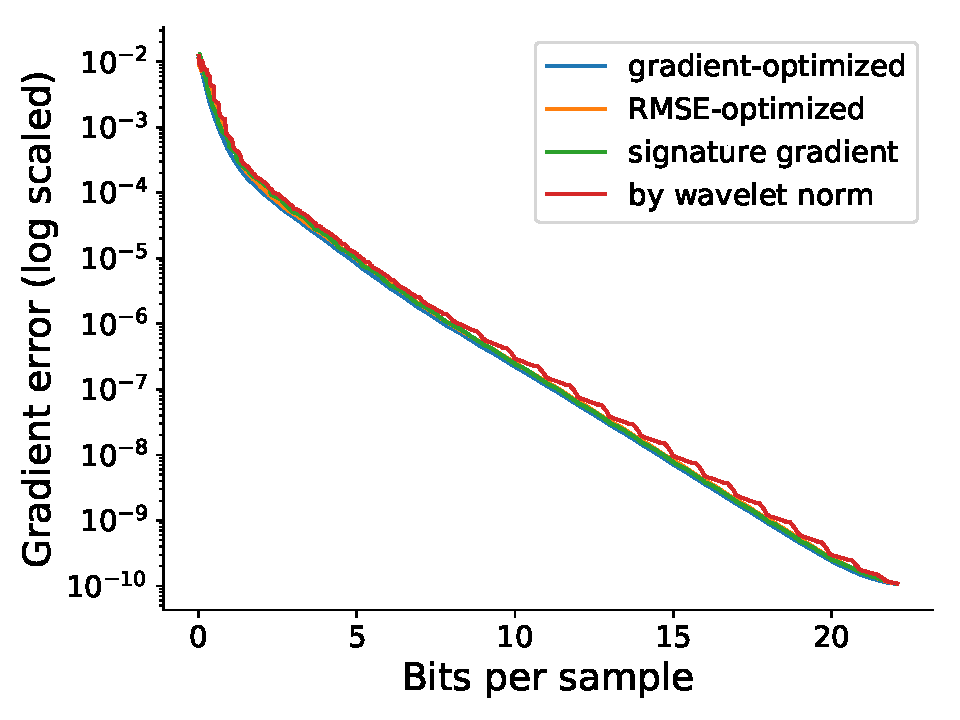
\includegraphics[width=0.48\linewidth]{img/gradient-laplacian/miranda-diffusivity-gradient-stencil-5.pdf}}
	\subcaptionbox{velocityz, 3-point stencil}
	{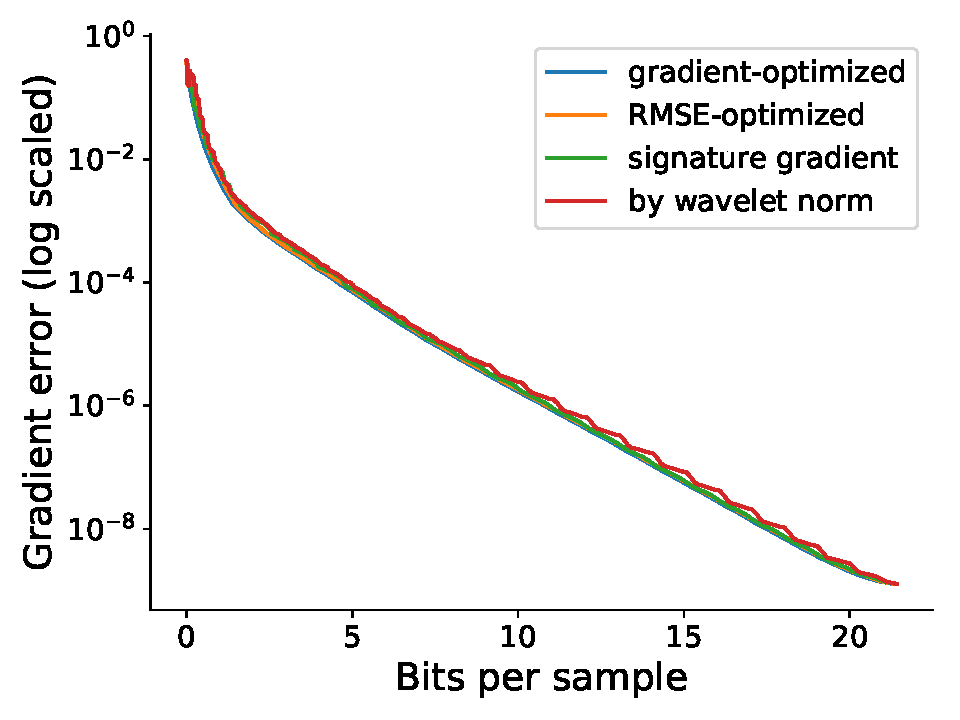
\includegraphics[width=0.48\linewidth]{img/gradient-laplacian/miranda-velocityz-gradient-stencil-3.pdf}}
	\subcaptionbox{velocityz, 5-point stencil}
	{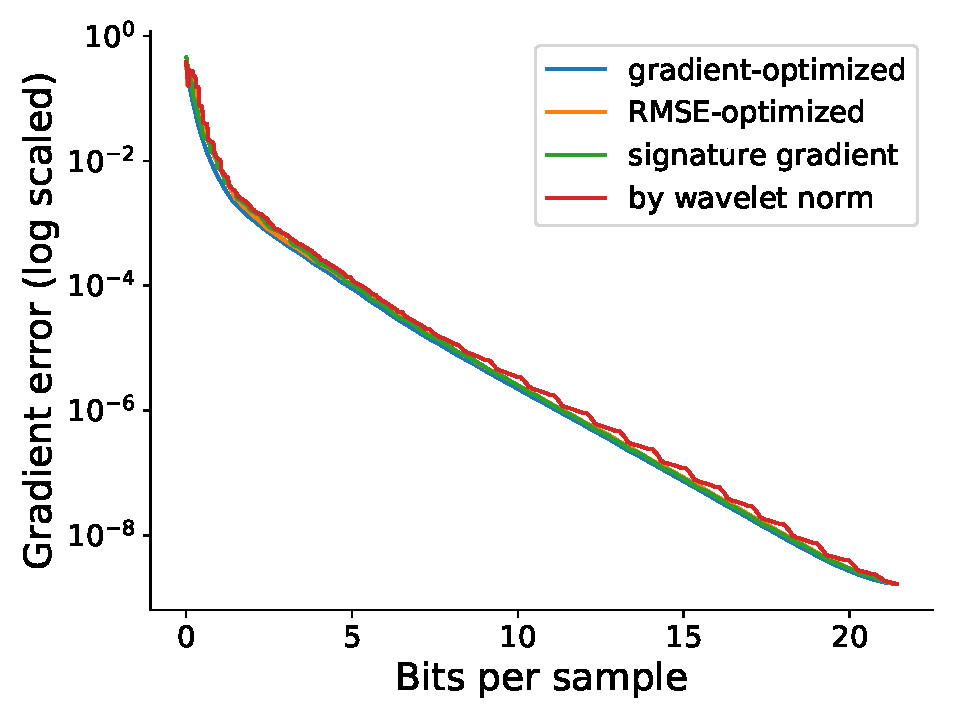
\includegraphics[width=0.48\linewidth]{img/gradient-laplacian/miranda-velocityz-gradient-stencil-5.pdf}}
	\caption{Gradient error comparison between \emph{gradient-optimized}, \emph{rmse-optimized},
	\emph{by wavelet norm}, and \emph{gradient signature} streams for four data sets, using the
	3-point stencil (left) and the 5-point stencil (right). Smaller is better. Chunks consisting of
	leading zero bits are removed from all streams. It all cases, the \emph{gradient-optimized} and
	\emph{rmse-optimized} streams perform the same, while \emph{gradient} signature is only slightly
	better than \emph{by wavelet norm}.}
	\label{fig:gradient-error-comparison}
\end{figure}

Figure \ref{fig:gradient-error-comparison} suggests that the \emph{rmse-optimized} streams are also
nearly optimal for gradient computation. The gradient operator is not invertible, that is, there are
infinitely many functions that result in the same gradient field. It is therefore not surprising
that the two streams both produce the best possible gradient progression. The \emph{rmse-optimized},
however, also produces an accurate function in addition to its gradient. We give evidence to this
claim is in Figure \ref{fig:gradient-comparison}, in which we reconstruct the euler data at $0.25$
bits per sample using both streams, and show the difference in gradient between the two. The two
gradient fields differ the most along very sharp edges, but are in general congruent (a), while the
\emph{rmse-optimized} stream produces significantly more accurate reconstruction of the function
itself (b, c, and d). It is therefore reasonable in practice to simply use \emph{by wavelet norm}
for the purpose of gradient computation.

\begin{figure}
	\centering
	\subcaptionbox{gradient difference}
	{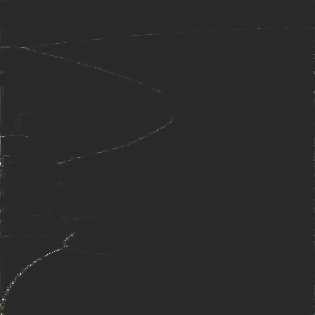
\includegraphics[width=0.24\linewidth]{img/gradient-laplacian/grad-diff.png}}
	\subcaptionbox{original data}
	{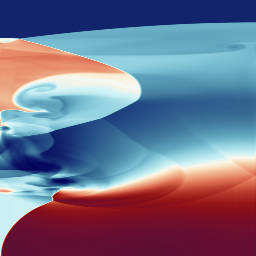
\includegraphics[width=0.24\linewidth]{img/gradient-laplacian/euler-original.png}}
	\subcaptionbox{\emph{rmse-optimized}}
	{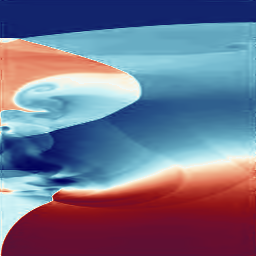
\includegraphics[width=0.24\linewidth]{img/gradient-laplacian/euler-rmse.png}}
	\subcaptionbox{\emph{gradient-optimized}, 3-point stencil}
	{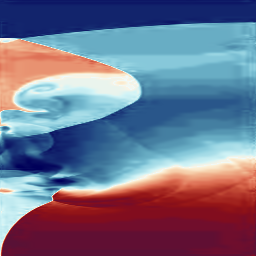
\includegraphics[width=0.24\linewidth]{img/gradient-laplacian/euler-gradient.png}}
	\caption{TODO: replace this figure (use 32-bit instead of 16-bit quantization). Comparing
	\emph{rmse-optimized} and \emph{gradient-optimized} at 0.25 bits per sample. }
	\label{fig:gradient-comparison}
\end{figure}

\subsection{Laplacian}

For Laplacian, we use the three-point finite difference in each dimension separately:
$\frac{{\partial}^2}{\partial{x^2}}f(x,y) \approx f(x-1,y)-2f(x,y)+f(x+1,y)$, and $\Delta
f=(\frac{{\partial}^2}{\partial{x^2}}+\frac{{\partial}^2}{\partial{y^2}})f$. The Laplacian error is
defined as the RMSE between the reconstructed Laplacian scalar field and the original Laplacian
scalar field. Again, algorithm [REF] is used to compute a \emph{laplacian-optimized} bit stream that
minimizes this error. In Figure \ref{fig:laplacian-comparison} we compare this stream with the
\emph{rmse-optimized} stream using the PSNR of the difference in Laplacian (compared to the
ground truth) as the error metric. The stream labeled \emph{laplacian signature} is to be ignored for
now. (TODO: why is it in the plot? maybe do not mention it at all? or just say that it will be explained later)

\begin{figure}
	\centering
	\subcaptionbox{euler}
	{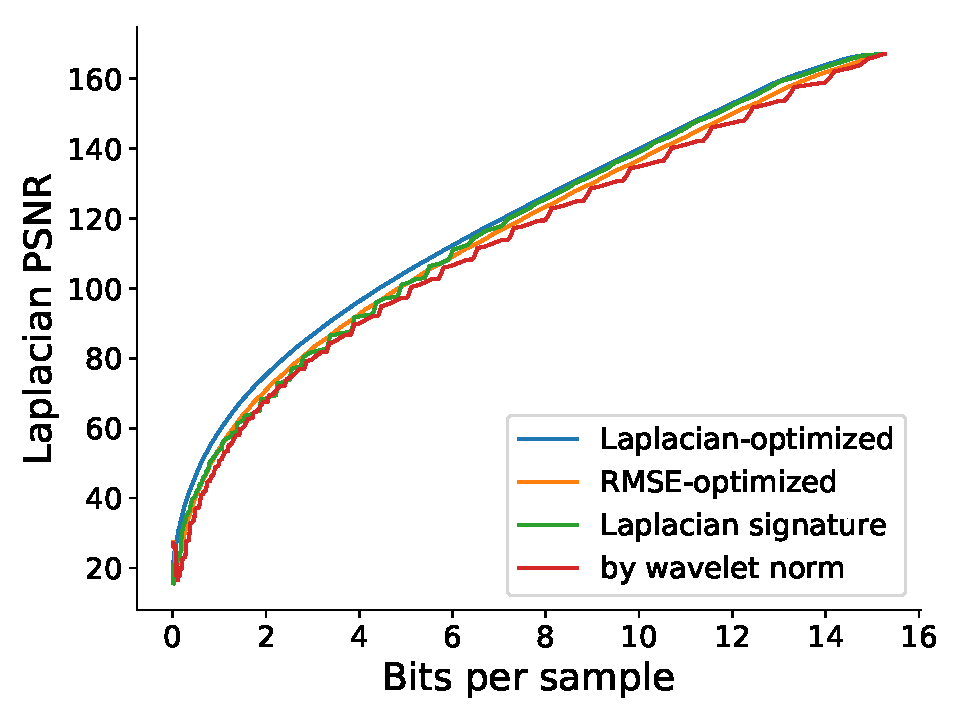
\includegraphics[width=0.48\linewidth]{img/gradient-laplacian/euler2d-laplacian.pdf}}
	\subcaptionbox{magnetic}
	{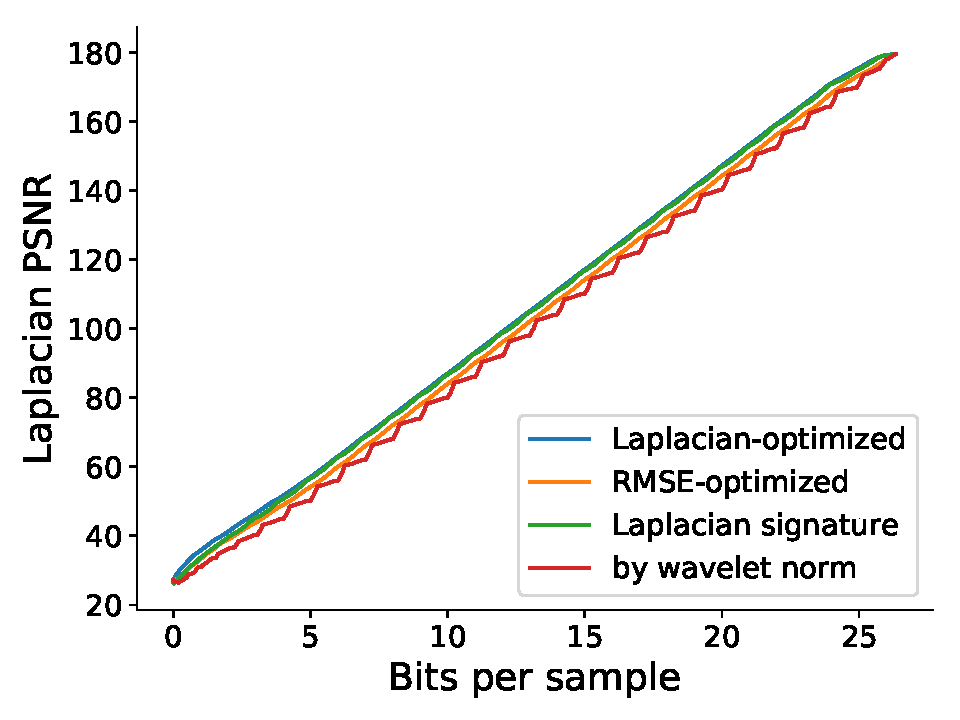
\includegraphics[width=0.48\linewidth]{img/gradient-laplacian/magnetic-laplacian.pdf}}
	\subcaptionbox{diffusivity}
	{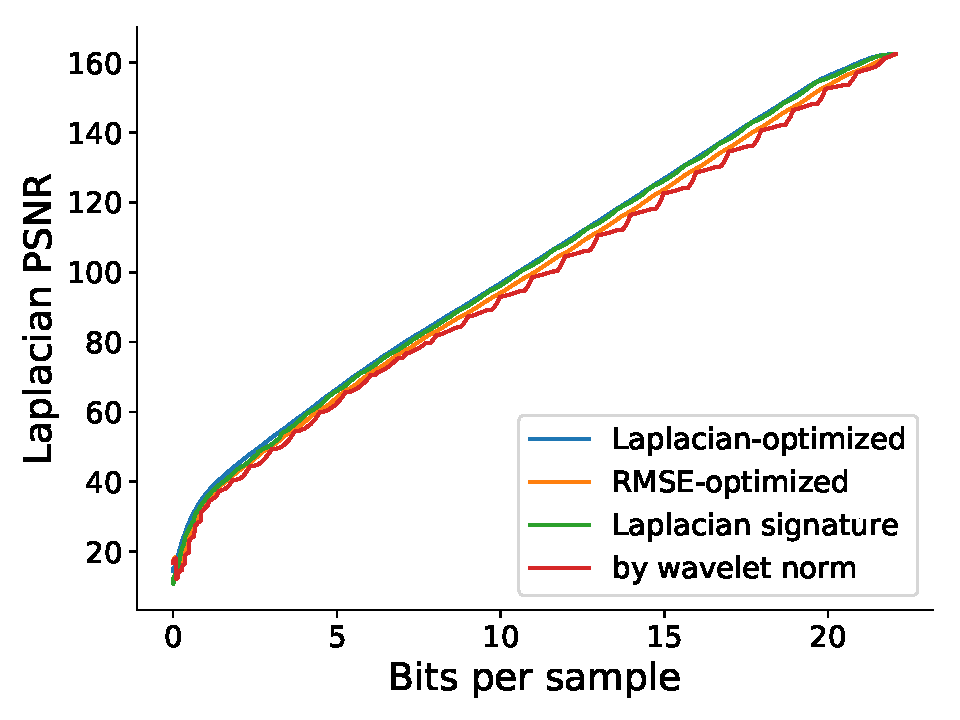
\includegraphics[width=0.48\linewidth]{img/gradient-laplacian/miranda-diffusivity-laplacian.pdf}}
	\subcaptionbox{velocityz}
	{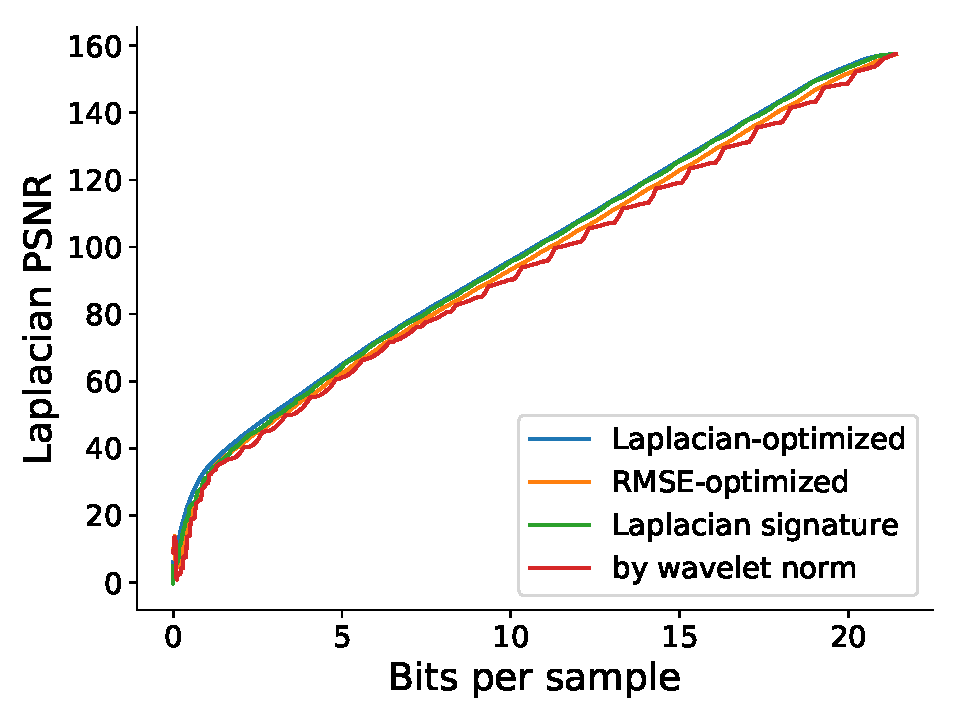
\includegraphics[width=0.48\linewidth]{img/gradient-laplacian/miranda-velocityz-laplacian.pdf}}
	\caption{Comparing \emph{rmse-optimized}, \emph{laplacian-optimized} and \emph{laplacian
	signature} streams in PSNR of Laplacian error (higher is better).}
	\label{fig:laplacian-comparison}
\end{figure}

It can be observed that unlike the case for gradient, there exists significant differences between
the \emph{rmse-optimized} and \emph{laplacian-optimized} streams with regards. To understand these
differences we plot the precision of every wavelet coefficients at a low bit rate in Figure
\ref{fig:laplacian-precision-comparison} (a and b). When cross refererencing this Figure with Figure
\ref{fig:gradient-comparison}b we see that the \emph{laplacian-optimized} stream priotizes
finer-resolution bits where the sharp shockwave is, unlike the \emph{rmse-optimized} stream which
prefers lower-ordered, coarse-resolution bits. This effect makes sense intuitively, as the
derivative operator makes functions less smooth, hence amplifing hard edges. This happens in the
gradient case too, but to a much lesser degree.

\begin{figure}
	\centering
	\subcaptionbox{\emph{laplacian-optimized}}
	{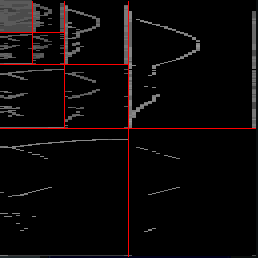
\includegraphics[width=0.32\linewidth]{img/gradient-laplacian/euler-prec-lap.png}}
	\subcaptionbox{\emph{rmse-optimized}}
	{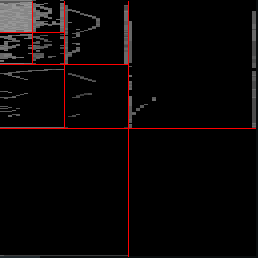
\includegraphics[width=0.32\linewidth]{img/gradient-laplacian/euler-prec-rmse.png}}
	\subcaptionbox{\emph{laplacian signature}}
	{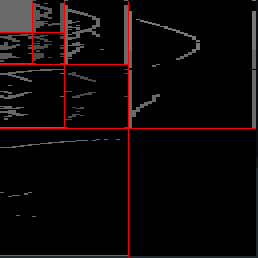
\includegraphics[width=0.32\linewidth]{img/gradient-laplacian/euler-prec-signature.png}}
	\caption{Precision distribution of wavelet coefficients at 0.25 bits per sample for the euler data
	set. Each square box with red boundary is a wavelet subband (the coarsest subband is in the top
	left). Brighter pixels correspond to higher-precision wavelet coefficients (black means no bit of
	that coefficient has not been received, while white means the whole coefficient has been
	received).}
	\label{fig:laplacian-precision-comparison}
\end{figure}

\emph{rmse-optimized}, \emph{laplacian-optimized}, and also \emph{gradient-optimized} for the euler
data set are visualized in Figure \ref{fig:signature-comparison}. 

\begin{figure}
	\centering
	\subcaptionbox{\emph{rmse-optimized}}
	{
\includegraphics[width=0.32\linewidth]{img/gradient-laplacian/SIG-GREEDY-(rmse).png}}
	\subcaptionbox{\emph{laplacian-optimized}}
	{
\includegraphics[width=0.32\linewidth]{img/gradient-laplacian/SIG-GREEDY-(laplacian).png}}
	\subcaptionbox{\emph{gradient-optimized}}
	{
\includegraphics[width=0.32\linewidth]{img/gradient-laplacian/SIG-GREEDY-(gradient).png}}
	\caption{Stream signatures visualized through a linear-blue color map (brighter is higher
	priority). From left to right: higher-ordered to lower-ordered bit planes. From top to bottom:
	coarser to finer subbands. Note that the streams from which the signatures are extracted do not
	contain leading zero bits, which explains the very dark cells }
	\label{fig:signature-comparison}
\end{figure}

Using the signature for \emph{laplacian-optimized}, we are able construct a data-independent stream
(in the sense that once the signature is computed and is given, the ordering of the bits follows the
the signature only). This stream, called \emph{laplacian signature}, performs at least as well as,
and often better, than \emph{rmse-optimized} for all data sets (see Figure
\ref{fig:laplacian-comparison}). The reason \emph{laplacian signature} does not always outperform
\emph{rmse-optimized}, and that there is still a gap between itself and \emph{laplacian-optimized}
is that the signature is computed essentially by `'averaging'' local signatures, a process that
lessen the effectiveness of the signature when the data is highly inhomogenous (e.g., the euler data
set with its sharp shockwaves). Nevertheless, even with one signature for the whole domain, we are
able to reconstruct more accurate Laplacian in all cases in experiment. In practice, the signature
is a tiny piece of meta information that can be pre-computed, stored, and transmitted before any
value bits to help `'steer'' the data stream, whenever Laplacian is the quantity of interest.
